\documentclass[aps,pra,twocolumn,superscriptaddress,nofootinbib,floatfix]{revtex4-2}

\usepackage{amsmath,amssymb,amsthm,bm}
\usepackage{mathtools}
\usepackage{graphicx}
\usepackage{xcolor}
\usepackage[colorlinks=true,linkcolor=blue!60!black,citecolor=blue!60!black,urlcolor=blue!60!black]{hyperref}

\graphicspath{{figures/}}

% ---------------------------------------------------------------------------
% Theorem environments and macros
% ---------------------------------------------------------------------------
\newtheorem{theorem}{Theorem}
\newtheorem{proposition}{Proposition}
\newtheorem{lemma}{Lemma}
\newtheorem{corollary}{Corollary}
\theoremstyle{definition}
\newtheorem{definition}{Definition}
\newtheorem{remark}{Remark}

\newcommand{\bra}[1]{\langle #1|}
\newcommand{\ket}[1]{|#1\rangle}
\newcommand{\tr}{\operatorname{tr}}
\DeclareMathOperator{\artanh}{artanh}
\newcommand{\vecr}{\vec r}
\newcommand{\mhat}{\hat m}
\newcommand{\nhat}{\hat n}
\newcommand{\vsigma}{\vec\sigma}
\newcommand{\maj}{\prec}
\newcommand{\omplus}{\omega_{\oplus}}
\newcommand{\omtimes}{\omega_{\otimes}}
\newcommand{\sqc}{\sqrt{c}}
\newcommand{\Ach}{\wp}
\newcommand{\todo}[1]{\textcolor{red}{[TODO: #1]}}

\begin{document}

\title{Uncertainty principles from majorization and entropy in the binary case}

\author{Rui Zhu}
\email{ruizhu2025@gmail.com}
\affiliation{Guangdong Technion -- Israel Institute of Technology, Shantou, Guangdong 515063, China}
% \todo{add co-authors / supervisors once agreed}

\date{\today}

\begin{abstract}
Majorization uncertainty relations bound the outcome statistics of all quantum
states by a single state-independent probability vector, and thereby bound
every Schur-concave uncertainty measure at once.
We give a self-contained treatment of the simplest non-trivial setting, a pair
of binary (two-outcome) measurements, and compare the majorization approach
systematically with entropy-specific uncertainty relations.
For projective qubit measurements with maximal overlap $c$, the direct-sum and
tensor-product bounds of the general theory reduce to
$\omplus=(1,\sqc,1-\sqc,0)$ and $\omtimes=(w,1-w,0,0)$ with $w=(1+\sqc)^2/4$.
Using the elliptical geometry of the achievable expectation values, we show
that these vectors are the least upper bounds of the achievable statistics in
the majorization lattice, that neither is attained unless the measurements
commute, and that their partial sums are saturated by two distinct families of
states.
Consequently, for non-commuting measurements every bound they imply for a
strictly Schur-concave measure---Shannon, R\'enyi of order $0<\alpha<\infty$,
Tsallis of order $q>0$---is strict; only the bounds of order $0$ and $\infty$
are attained.
We map out, across the R\'enyi family, when the direct-sum or the
tensor-product form is preferable and how both compare with the
Maassen--Uffink relation and with the exact optimum.
Finally, we give the optimal direct-sum bound for arbitrary unsharp and biased
two-outcome qubit POVMs, discuss its relation to joint measurability, and use
Jordan's lemma to extend the projective results to binary projective
measurements in any finite dimension.
\end{abstract}

\maketitle

% ===========================================================================
\section{Introduction}
\label{sec:intro}
% ===========================================================================

The uncertainty principle~\cite{Heisenberg1927,Robertson1929} expresses the
impossibility of preparing a quantum state that yields sharp outcomes for two
incompatible measurements.
Its information-theoretic formulation replaces variances by entropies of the
outcome distributions $p$ and $q$ of two measurements $M$ and $N$~\cite{Deutsch1983,Kraus1987,MaassenUffink1988}.
The best known example is the Maassen--Uffink (MU) relation~\cite{MaassenUffink1988}
\begin{equation}
  H(p)+H(q)\;\geq\;-\log_2 c,\qquad c=\max_{i,j}|\langle m_i|n_j\rangle|^2 ,
  \label{eq:MU}
\end{equation}
which has become a workhorse of quantum cryptography and quantum information
theory~\cite{WehnerWinter2010,Coles2017} and has been improved in various
regimes~\cite{deVicente2008,ColesPiani2014}.

A scalar inequality such as~\eqref{eq:MU} constrains one particular functional
of the pair $(p,q)$; a different uncertainty measure requires a different
relation.
Majorization~\cite{MarshallOlkin2011} provides a structural alternative.
One seeks a single state-independent probability vector $\omega$ such that
\begin{equation}
  p(\rho)\oplus q(\rho)\;\maj\;\omega
  \quad\text{or}\quad
  p(\rho)\otimes q(\rho)\;\maj\;\omega
  \qquad\forall\rho ,
  \label{eq:maj-UR}
\end{equation}
so that every Schur-concave function $\Phi$---Shannon, R\'enyi or Tsallis entropies,
among many others---inherits the bound $\Phi(p\oplus q)\ge\Phi(\omega)$
automatically.
This programme was initiated by Partovi~\cite{Partovi2011} and developed into
universal uncertainty relations of tensor-product form by Friedland, Gheorghiu
and Gour~\cite{FGG2013} and by Pucha{\l}a, Rudnicki and
{\.Z}yczkowski~\cite{PRZ2013}; the direct-sum form, which yields stronger
entropic bounds, was introduced in Ref.~\cite{RPZ2014}.
It has since been extended to POVMs and quantum
operations~\cite{RasteginZyczkowski2016,Baek2019} and sharpened
further~\cite{Li2016,Yuan2023}, in particular by exploiting the lattice
structure of majorization~\cite{Yuan2023}.

For a qubit, entropy-specific relations can be pushed further: the optimal
Shannon relation for two projective measurements is
known~\cite{SanchezRuiz1998,Ghirardi2003}, and so are optimal relations for
R\'enyi entropies~\cite{BosykPortesiPlastino2012,ZozorBosykPortesi2013}.
This raises a natural question: in the simplest setting, where both approaches
can be carried out completely, what exactly does majorization gain, and what
does it cost?

In this paper we answer this question for binary (two-outcome) measurements.
Several ingredients are known. For two qubit bases, the vectors $\omplus$ and
$\omtimes$ of Sec.~\ref{sec:projective} are the $d=2$ instances of the bounds of
Refs.~\cite{RPZ2014} and~\cite{PRZ2013,FGG2013}, and for unbiased unsharp qubit
observables the direct-sum bound was evaluated in Ref.~\cite{Baek2019}.
Building on these results, we give a unified and self-contained treatment of the
binary case:
\begin{enumerate}
  \item[(i)] From the elliptical geometry of the achievable expectation values
    (Lemma~\ref{lem:ellipse}) we derive both bounds, prove that they are the
    least upper bounds of the achievable statistics in the majorization
    lattice, show that neither is attained unless the measurements commute, and
    identify the two families of states that saturate their partial sums
    (Sec.~\ref{sec:projective}).
  \item[(ii)] We characterize when the resulting entropic bounds are tight: for
    non-commuting measurements every bound for a strictly Schur-concave
    measure is strict, and only the bounds of order $0$ and $\infty$ are
    attained (Theorem~\ref{thm:tight}).
  \item[(iii)] We compare the direct-sum and tensor-product forms with each
    other, with MU and with the exact optimum across the whole R\'enyi family
    (Sec.~\ref{sec:entropic}).
  \item[(iv)] We obtain the optimal direct-sum bound for arbitrary unsharp and
    biased two-outcome qubit POVMs and discuss its relation to joint
    measurability (Sec.~\ref{sec:povm}), and we extend the projective results
    to binary projective measurements in any finite dimension
    (Sec.~\ref{sec:dimd}).
\end{enumerate}
All statements are checked numerically with the accompanying code
(Appendix~\ref{app:numerics}).

% ===========================================================================
\section{Preliminaries}
\label{sec:prelim}
% ===========================================================================

\subsection{Majorization and uncertainty measures}

For $x\in\mathbb{R}^d$ let $x^\downarrow$ denote its entries in non-increasing
order and $L_k(x)=\sum_{i=1}^k x^\downarrow_i$ its Lorenz partial sums.
For $x,y$ with equal total, $x$ is \emph{majorized} by $y$, written $x\maj y$,
if $L_k(x)\le L_k(y)$ for all $k$~\cite{MarshallOlkin2011}.
A function $\Phi$ is Schur-concave if $x\maj y$ implies $\Phi(x)\ge\Phi(y)$,
and \emph{strictly} Schur-concave if, in addition, $\Phi(x)>\Phi(y)$ whenever
$x\maj y$ and $x^\downarrow\neq y^\downarrow$.
Every function $\Phi(x)=\sum_i\phi(x_i)$ with $\phi$ (strictly) concave is
(strictly) Schur-concave~\cite{MarshallOlkin2011}.

The uncertainty measures used below are the R\'enyi~\cite{Renyi1961} and
Tsallis~\cite{Tsallis1988} entropies
\begin{equation}
  H_\alpha(p)=\frac{\log_2\sum_ip_i^\alpha}{1-\alpha},\qquad
  T_q(p)=\frac{1-\sum_ip_i^q}{q-1},
  \label{eq:entropies}
\end{equation}
with the Shannon entropy $H=H_1$ as the common limit ($T_q\to H\ln2$ as
$q\to1$). The orders $\alpha=\infty$ and $\alpha=\frac12$ give the min-entropy
$H_\infty(p)=-\log_2\max_ip_i$ and the max-entropy $H_{1/2}$, and $H_0$ is the
logarithm of the number of non-zero entries.
All of them are Schur-concave; $H_\alpha$ is strictly Schur-concave for
$0<\alpha<\infty$ and $T_q$ for $q>0$, whereas $H_0$ and $H_\infty$ are not.

Restricted to non-increasing vectors of fixed total, $\maj$ is a partial order,
and in fact a complete lattice~\cite{CicaleseVaccaro2002,Bosyk2019}.

\begin{definition}
Let $A$ be a set of vectors with common total. A vector $\omega$ is an
\emph{optimal majorization bound} for $A$ if $a\maj\omega$ for all $a\in A$, and
$\omega\maj\omega'$ for every other $\omega'$ with this property; i.e.,
$\omega=\sup A$ in the majorization lattice.
\end{definition}

\begin{lemma}[\cite{CicaleseVaccaro2002,Bosyk2019}]
\label{lem:sup}
Let $S_k=\sup_{a\in A}L_k(a)$. Then $\sup A$ is the vector whose Lorenz curve is
the least concave majorant of $k\mapsto S_k$ (with $S_0=0$). In particular, if
$\omega_k=S_k-S_{k-1}$ is already non-increasing, then $\omega=\sup A$.
\end{lemma}

In all cases treated below the second, simpler statement applies.
The quantities $S_k$ have a transparent meaning: $S_k$ is the largest total
probability that any state can concentrate on $k$ outcomes.

\subsection{Two-outcome qubit measurements}

A qubit state is $\rho=\tfrac12(\mathbb{1}+\vecr\cdot\vsigma)$ with $|\vecr|\le1$.
A projective two-outcome measurement is $M=\{P_\pm\}$ with
$P_\pm=\tfrac12(\mathbb{1}\pm\mhat\cdot\vsigma)$, $|\mhat|=1$, and similarly
$N=\{Q_\pm\}$ with axis $\nhat$.
The outcome distributions are
\begin{equation}
  p=\Bigl(\tfrac{1+x}{2},\tfrac{1-x}{2}\Bigr),\;
  q=\Bigl(\tfrac{1+y}{2},\tfrac{1-y}{2}\Bigr),\quad
  x=\mhat\cdot\vecr,\; y=\nhat\cdot\vecr .
  \label{eq:pq}
\end{equation}
The overlaps are $|\langle m_\pm|n_\pm\rangle|^2=\tfrac12(1+\mhat\cdot\nhat)$ and
$|\langle m_\pm|n_\mp\rangle|^2=\tfrac12(1-\mhat\cdot\nhat)$, hence
\begin{equation}
  c=\tfrac12\bigl(1+|\mhat\cdot\nhat|\bigr)=\cos^2\tfrac{\theta}{2},
  \qquad \cos\theta=|\mhat\cdot\nhat|,\;\theta\in[0,\tfrac{\pi}{2}] .
  \label{eq:c}
\end{equation}
Relabelling the outcomes of $N$ maps $\nhat\mapsto-\nhat$ and does not affect any
majorization statement, so we may and shall assume $\mhat\cdot\nhat=\cos\theta\ge0$.
Note that $\tfrac12\le c\le1$ and $\sqc\ge1/\sqrt2>1-\sqc$.

A general two-outcome POVM $\{E_0,E_1=\mathbb{1}-E_0\}$ can always be written as
\begin{equation}
  E_0=\tfrac12\bigl[(1+\mu)\mathbb{1}+\eta\,\hat a\cdot\vsigma\bigr],
  \qquad \eta\ge0,\;|\mu|+\eta\le1 ,
  \label{eq:povm}
\end{equation}
the constraint being equivalent to $0\le E_0\le\mathbb{1}$.
Here $\eta$ is the sharpness and $\mu$ the bias; rank-one projective
measurements correspond to $\eta=1$, $\mu=0$.

% ===========================================================================
\section{Geometry of the achievable set}
\label{sec:geometry}
% ===========================================================================

The statistics~\eqref{eq:pq} depend on $\vecr$ only through $(x,y)$.

\begin{lemma}
\label{lem:ellipse}
For non-parallel axes, the set $\{(\mhat\cdot\vecr,\nhat\cdot\vecr):|\vecr|\le1\}$ is the
filled ellipse
\begin{equation}
  \mathcal{E}_\theta=\bigl\{(x,y): x^2-2xy\cos\theta+y^2\le\sin^2\theta\bigr\}.
\end{equation}
Its boundary consists exactly of the images of the pure states whose Bloch
vectors lie in $\mathrm{span}\{\mhat,\nhat\}$. Moreover, for all $\alpha,\beta\in\mathbb{R}$,
\begin{equation}
  \max_{|\vecr|\le1}\,(\alpha x+\beta y)=|\alpha\mhat+\beta\nhat| .
  \label{eq:support}
\end{equation}
\end{lemma}

\begin{proof}
Write $\vecr=\vec r_\parallel+\vec r_\perp$ with $\vec r_\parallel\in\mathrm{span}\{\mhat,\nhat\}$.
Only $\vec r_\parallel$ contributes to $(x,y)$, and $(x,y)=G\,\xi$ where $\xi$ are the
coefficients of $\vec r_\parallel$ in the basis $\{\mhat,\nhat\}$ and
$G=\bigl(\begin{smallmatrix}1&\cos\theta\\ \cos\theta&1\end{smallmatrix}\bigr)$
is the Gram matrix. Then $|\vec r_\parallel|^2=\xi^TG\xi=(x,y)G^{-1}(x,y)^T\le1$,
which is the stated inequality since $\det G=\sin^2\theta$. Equality holds iff
$\vec r_\perp=0$ and $|\vecr|=1$. Eq.~\eqref{eq:support} is Cauchy--Schwarz:
$\alpha x+\beta y=\vecr\cdot(\alpha\mhat+\beta\nhat)$.
\end{proof}

Consequently the achievable set
$\Ach(M,N)=\{p(\rho)\oplus q(\rho)\}\subset\mathbb{R}^4$ is the image of
$\mathcal{E}_\theta$ under the affine map
$(x,y)\mapsto\tfrac12(1+x,1-x,1+y,1-y)$: it is convex and compact, and its
extreme points are the statistics of pure states in the plane of the two axes
(Fig.~\ref{fig:ellipse}). Any uncertainty measure that is concave in $(x,y)$,
such as $H(p)+H(q)$, is therefore minimized on $\partial\mathcal{E}_\theta$, and
the optimization problems below are effectively one-dimensional.

\begin{figure}[t]
  \centering
  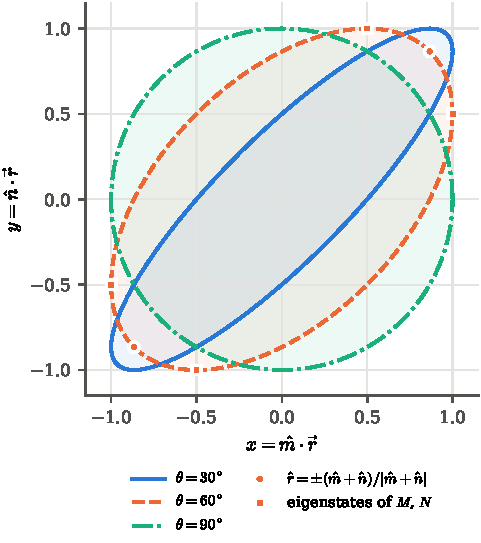
\includegraphics[width=\columnwidth]{achievable_set.pdf}
  \caption{The ellipse $\mathcal{E}_\theta$ of achievable expectation values
  $(x,y)=(\langle\mhat\cdot\vsigma\rangle,\langle\nhat\cdot\vsigma\rangle)$ for three
  Bloch angles. Markers (for $\theta=60^\circ$) show the two families of states
  that saturate the partial sums of $\omplus$: eigenstates of $M$ or $N$
  (squares; $k=1,3$) and bisector states $\hat r\propto\pm(\mhat+\nhat)$
  (circles; $k=2$). No single point saturates all partial sums
  (Proposition~\ref{prop:attain}).}
  \label{fig:ellipse}
\end{figure}

% ===========================================================================
\section{Projective measurements}
\label{sec:projective}
% ===========================================================================

\subsection{Direct-sum bound}

\begin{theorem}
\label{thm:direct}
Let $M,N$ be projective qubit measurements with maximal overlap $c$. For every
state $\rho$,
\begin{equation}
  p(\rho)\oplus q(\rho)\;\maj\;\omplus:=\bigl(1,\;\sqc,\;1-\sqc,\;0\bigr),
  \label{eq:omplus}
\end{equation}
and $\omplus$ is the optimal majorization bound for $\Ach(M,N)$.
\end{theorem}

The majorization relation~\eqref{eq:omplus} is the qubit case of the direct-sum
relation $p\oplus q\maj\{1\}\oplus W$ of Rudnicki \emph{et al.}~\cite{RPZ2014}:
for $d=2$ their vector $W=(s_1,s_2-s_1)$ has $s_1=\sqc$ and $s_2=1$. We give a
short proof based on Lemma~\ref{lem:ellipse}, which also yields optimality and
the maximizing states.

\begin{proof}
We compute $S_k=\max_\rho L_k(p\oplus q)$ for $k=1,\dots,4$.
Clearly $S_1\le1$ and $S_4=2$. Since all entries are non-negative,
$S_3=2-\min_\rho\min_i(p\oplus q)_i\le2$.
Both bounds are attained by an eigenstate of $M$, for which $p=(1,0)$.
For $k=2$, the two largest entries either belong to the same distribution, with
sum $1$, or are of the form $p_i+q_j$. By Lemma~\ref{lem:ellipse},
\begin{equation}
  p_i+q_j=1+\tfrac12(\pm x\pm y)\le1+\tfrac12\max\{|\mhat+\nhat|,|\mhat-\nhat|\}.
\end{equation}
With $\mhat\cdot\nhat=\cos\theta\ge0$ the maximum is
$|\mhat+\nhat|=\sqrt{2(1+\cos\theta)}=2\cos\frac\theta2=2\sqc$, so
\begin{equation}
  S_2=1+\sqc ,
  \label{eq:S2}
\end{equation}
attained by the bisector state $\vecr=(\mhat+\nhat)/|\mhat+\nhat|$. This is the qubit case
of the Landau--Pollak-type inequality $p_i+q_j\le1+\sqc$ underlying Deutsch's
relation~\cite{LandauPollak1961,Deutsch1983}. The increments of $(S_1,S_2,S_3,S_4)=(1,1+\sqc,2,2)$
give $\omplus$, which is non-increasing because $1\ge\sqc\ge1-\sqc\ge0$.
Lemma~\ref{lem:sup} completes the proof.
\end{proof}

\begin{proposition}
\label{prop:attain}
There is a state with $(p\oplus q)^\downarrow=\omplus$ if and only if $c=1$,
i.e., $M$ and $N$ commute. For $c<1$, the maxima $S_1,S_3$ are attained only by
the eigenstates of $M$ and $N$, and $S_2$ only by the bisector states
$\vecr=\pm(\mhat+\nhat)/|\mhat+\nhat|$ (for $\theta=\pi/2$ also by
$\vecr=\pm(\mhat-\nhat)/|\mhat-\nhat|$).
\end{proposition}

\begin{proof}
$(p\oplus q)^\downarrow_1=1$ forces $\rho$ to be an eigenstate of $M$ or $N$, say
$\vecr=\pm\mhat$. Then $q=\bigl(\frac{1\pm\cos\theta}{2},\frac{1\mp\cos\theta}{2}\bigr)$ and
$(p\oplus q)^\downarrow=(1,c,1-c,0)$, which equals $\omplus$ iff $c=\sqc$, i.e.,
$c=1$. The statement about $S_2$ follows from the equality condition in
Cauchy--Schwarz and from $|\mhat-\nhat|<|\mhat+\nhat|$ for $\theta<\pi/2$.
\end{proof}

Proposition~\ref{prop:attain} makes precise the sense in which $\omplus$ is a
\emph{description} of the achievable set rather than the statistics of a
particular state: it is the supremum of $\Ach(M,N)$ in the majorization
lattice, and its partial sums are saturated by two disjoint families of states
(Fig.~\ref{fig:lorenz}). The gap between
$(1,c,1-c,0)$ and $\omplus$ quantifies the price one pays for demanding
certainty about $M$.

\begin{figure}[t]
  \centering
  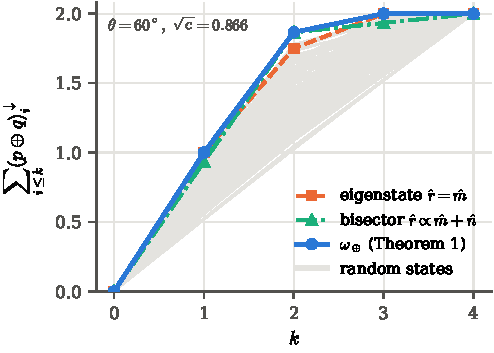
\includegraphics[width=\columnwidth]{lorenz.pdf}
  \caption{Lorenz curves of $p\oplus q$ for $\theta=60^\circ$. Grey: 150 random
  states. The optimal bound $\omplus$ (blue) is the upper envelope; it touches
  the eigenstate curve at $k=1,3$ and the bisector-state curve at $k=2$, but no
  single state reaches it.}
  \label{fig:lorenz}
\end{figure}

\subsection{Tensor-product bound}

\begin{theorem}
\label{thm:tensor}
For every state $\rho$,
\begin{equation}
  p(\rho)\otimes q(\rho)\;\maj\;\omtimes:=\bigl(w,\;1-w,\;0,\;0\bigr),
  \label{eq:omtimes}
\end{equation}
where $w=\frac14\bigl(1+\sqc\bigr)^2$, and $\omtimes$ is the optimal
majorization bound for $\{p(\rho)\otimes q(\rho)\}$.
\end{theorem}

The vector $\omtimes$ coincides with the vector $Q^{(1)}=(C^2,1-C^2,0,0)$,
$C=(1+\sqc)/2$, of Pucha{\l}a \emph{et al.}~\cite{PRZ2013}, which for $d=2$
exhausts their hierarchy of bounds; see also Ref.~\cite{FGG2013}.

\begin{proof}
By the arithmetic--geometric mean inequality and Eq.~\eqref{eq:S2},
$p_iq_j\le\bigl(\tfrac{p_i+q_j}{2}\bigr)^2\le\bigl(\tfrac{1+\sqc}{2}\bigr)^2=w$,
with equality for the bisector state, for which $p_+=q_+=(1+\sqc)/2$.
Hence $S_1=w$. For an eigenstate of $M$, $p\otimes q=(q_+,q_-,0,0)$, so
$S_2=S_3=S_4=1$. Since $\sqc\ge1/\sqrt2$ we have $w\ge\frac12$, so the increments
$(w,1-w,0,0)$ are non-increasing, and Lemma~\ref{lem:sup} applies.
\end{proof}

As before, $\omtimes$ is not attained for $c<1$: equality in both steps of the
proof forces a bisector state, at which $L_2(p\otimes q)=p_+=(1+\sqc)/2<1$.

% ===========================================================================
\section{Entropic uncertainty relations}
\label{sec:entropic}
% ===========================================================================

Let $h(t)=-t\log_2t-(1-t)\log_2(1-t)$ be the binary entropy.

\subsection{Bounds for the R\'enyi and Tsallis families}

\begin{corollary}
\label{cor:direct}
For every concave $\phi$ on $[0,1]$,
$\sum_i\phi(p_i)+\sum_j\phi(q_j)\ge\phi(1)+\phi(\sqc)+\phi(1-\sqc)+\phi(0)$.
In particular,
\begin{align}
  H(p)+H(q)&\;\ge\;h(\sqc) ,
  \label{eq:Hdirect}\\
  T_q(p)+T_q(q)&\;\ge\;\frac{1-c^{q/2}-(1-\sqc)^q}{q-1}\qquad(q>0),
  \label{eq:Tdirect}
\end{align}
and, for $0<\alpha\le1$,
\begin{equation}
  H_\alpha(p)+H_\alpha(q)\;\ge\;H_\alpha(\sqc,1-\sqc),
  \label{eq:Rdirect}
\end{equation}
where $H_\alpha(\sqc,1-\sqc)=\log_2\bigl[c^{\alpha/2}+(1-\sqc)^\alpha\bigr]/(1-\alpha)$.
\end{corollary}

\begin{proof}
The first statement is Karamata's inequality applied to Theorem~\ref{thm:direct}.
Eqs.~\eqref{eq:Hdirect} and~\eqref{eq:Tdirect} follow with $\phi(t)=-t\log_2t$
and $\phi_q(t)=(t-t^q)/(q-1)$, since $\sum_ip_i=\sum_jq_j=1$ gives
$T_q(p)+T_q(q)=\sum_k\phi_q\bigl((p\oplus q)_k\bigr)$.
Eq.~\eqref{eq:Rdirect} is the qubit case of Theorem~2 of Ref.~\cite{RPZ2014};
we recall the short argument. For $\alpha<1$ write $\sum_ip_i^\alpha=1+A$ and
$\sum_jq_j^\alpha=1+B$ with $A,B\ge0$. Then
\begin{align*}
  H_\alpha(p)+H_\alpha(q)&=\frac{\log_2[(1+A)(1+B)]}{1-\alpha}\\
  &\ge\frac{\log_2(1+A+B)}{1-\alpha},
\end{align*}
and $1+A+B=\sum_k(p\oplus q)_k^\alpha-1\ge\sum_k(\omplus)_k^\alpha-1=c^{\alpha/2}+(1-\sqc)^\alpha$
by Schur-concavity of $v\mapsto\sum_kv_k^\alpha$.
\end{proof}

\begin{corollary}
\label{cor:tensor}
For every $\alpha\in[0,\infty]$,
\begin{equation}
  H_\alpha(p)+H_\alpha(q)\;\ge\;H_\alpha(\omtimes)=\frac{\log_2\!\bigl[w^\alpha+(1-w)^\alpha\bigr]}{1-\alpha}.
  \label{eq:Rtensor}
\end{equation}
For $\alpha=1$ this reads $H(p)+H(q)\ge h(w)$; for $\alpha=\infty$ it gives
$H_\infty(p)+H_\infty(q)\ge-2\log_2\frac{1+\sqc}{2}$, which is tight (bisector
state); since $H\ge H_\infty$, it contains Deutsch's Shannon
bound~\cite{Deutsch1983}, which has the same right-hand side.
\end{corollary}

The two forms are natural for different families: Tsallis entropies are
additive over direct sums, as used in the proof of Corollary~\ref{cor:direct},
whereas R\'enyi entropies are additive over tensor products,
$H_\alpha(p\otimes q)=H_\alpha(p)+H_\alpha(q)$. Where both forms apply, the
direct sum is stronger, but it cannot be extended to all orders:

\begin{proposition}
\label{prop:compare}
(i) For $0<\alpha\le1$, $H_\alpha(\sqc,1-\sqc)\ge H_\alpha(\omtimes)$, with
equality iff $c=1$; in particular $h(\sqc)\ge h(w)$.
(ii) For $c<1$ the direct-sum form~\eqref{eq:Rdirect} fails at $\alpha=\infty$:
$\min_\rho[H_\infty(p)+H_\infty(q)]=-2\log_2\frac{1+\sqc}{2}<-\frac12\log_2c=H_\infty(\sqc,1-\sqc)$.
\end{proposition}

\begin{proof}
(i) Since $w-\sqc=\frac14(1-\sqc)^2\ge0$, we have $(\sqc,1-\sqc)\maj(w,1-w)$,
with equality iff $c=1$; apply strict Schur-concavity. The analogous statement
in any dimension is proven in Ref.~\cite{RPZ2014}.
(ii) With $t=\sqc$, $\bigl(\frac{1+t}{2}\bigr)^2-t=\bigl(\frac{1-t}{2}\bigr)^2>0$
for $t<1$; the minimum is the tight bound of Corollary~\ref{cor:tensor}.
\end{proof}

\subsection{When are the bounds tight?}

\begin{theorem}
\label{thm:tight}
Let $c<1$.
(i) For every continuous, strictly Schur-concave $\Phi$,
\begin{equation}
  \min_\rho\Phi(p\oplus q)>\Phi(\omplus),\qquad
  \min_\rho\Phi(p\otimes q)>\Phi(\omtimes).
\end{equation}
Consequently the bounds~\eqref{eq:Hdirect}, \eqref{eq:Tdirect}
and~\eqref{eq:Rdirect}, and the bounds~\eqref{eq:Rtensor} with
$0<\alpha<\infty$, are all strict.
(ii) The bounds~\eqref{eq:Rtensor} of order $\alpha=0$ and $\alpha=\infty$ are
tight; they are attained by the eigenstates of $M$ or $N$ and by the bisector
states, respectively.
\end{theorem}

\begin{proof}
(i) The achievable statistics form a compact set, so the minimum of $\Phi$ is
attained at some state $\rho^\ast$. By Theorem~\ref{thm:direct} and
Proposition~\ref{prop:attain}, $p\oplus q(\rho^\ast)\maj\omplus$ with
$(p\oplus q)^\downarrow\neq\omplus$, hence $\Phi(p\oplus q(\rho^\ast))>\Phi(\omplus)$.
The tensor product is analogous, using the non-attainment of $\omtimes$ shown
after Theorem~\ref{thm:tensor}. The Shannon and Tsallis sums are strictly
Schur-concave functions of $p\oplus q$, and $H_\alpha(p)+H_\alpha(q)=H_\alpha(p\otimes q)$
with $H_\alpha$ strictly Schur-concave for $0<\alpha<\infty$. For~\eqref{eq:Rdirect}
with $\alpha<1$, apply the argument to $v\mapsto\sum_kv_k^\alpha$ in the proof of
Corollary~\ref{cor:direct}.
(ii) An eigenstate of $M$ gives $H_0(p)+H_0(q)=0+1=H_0(\omtimes)$, and a bisector
state gives $\max_ip_i\max_jq_j=w$.
\end{proof}

Theorem~\ref{thm:tight} makes precise in what sense the majorization bounds are
optimal. As majorization bounds they cannot be improved
(Theorems~\ref{thm:direct} and~\ref{thm:tensor}); yet, because the supremum is
not the statistics of any state, the bound it induces is strict for every
strictly Schur-concave measure. For such measures the optimum has to be found
measure by measure, which is what entropy-specific relations do; only at the
extreme orders $\alpha=0$ and $\alpha=\infty$ does the majorization bound reach
it.

\subsection{Comparison with the Maassen--Uffink relation and with the exact optimum}

Figure~\ref{fig:entropic} compares the Shannon bounds with MU and with the
exact minimum of $H(p)+H(q)$, which is known for
qubits~\cite{SanchezRuiz1998,Ghirardi2003}. By Lemma~\ref{lem:ellipse} the
minimum lies on the great circle through $\mhat$ and $\nhat$. For
$\theta\le\bar\theta$ it is attained at the bisector states and equals
$2h\bigl(\frac{1+\sqc}{2}\bigr)$~\cite{Ghirardi2003}. At $\bar\theta$ the
bisector turns from a minimum into a saddle point along the circle; a
second-derivative test shows that this happens when
$\sqrt{\bar c}\,\artanh\sqrt{\bar c}=1$, i.e., at $\bar c\approx0.6948$ and
$\bar\theta\approx67.07^\circ$. For $\bar\theta<\theta<\pi/2$ the minimizers
bifurcate and the minimum has to be computed numerically~\cite{Ghirardi2003}.

For mutually unbiased measurements ($\theta=90^\circ$, $c=\frac12$) MU is tight
(1 bit), while $h(1/\sqrt2)\approx0.872$ and $h(w)\approx0.844$. As the
measurements become more compatible, however, the majorization bounds take
over: $h(\sqc)>-\log_2c$ for $\sqc>t^\ast\approx0.7585$, i.e., for Bloch angles
$\theta<81.3^\circ$ (the tensor bound overtakes MU at $\theta<79.3^\circ$), in
agreement with Ref.~\cite{Baek2019}.

As $c\to1$ the advantage over MU becomes unbounded, and the direct-sum bound
becomes tight in ratio. With $\varepsilon=1-\sqc\approx\theta^2/8$ one has
$-\log_2c\approx2\varepsilon/\ln2$ and
$h(\sqc)=h(\varepsilon)\approx\varepsilon\log_2(e/\varepsilon)$, whereas the
exact minimum is $2h(\varepsilon/2)\approx\varepsilon\log_2(2e/\varepsilon)$.
To leading order the ratio of the exact minimum to $h(\sqc)$ is therefore
$1+1/\log_2(e/\varepsilon)$: it tends to $1$, but only logarithmically ($1.09$
at $\theta=0.1$, $1.047$ at $\theta=0.003$), while the ratio to MU grows as
$\frac12\ln(16e/\theta^2)$ ($4.2$ and $7.7$). The eigenstates of $M$, although
they saturate $S_1$ and $S_3$, give $h(c)$, asymptotically twice the minimum.

\begin{figure}[t]
  \centering
  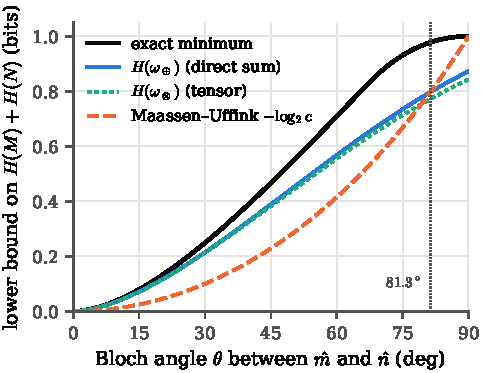
\includegraphics[width=\columnwidth]{entropic_bounds.pdf}
  \caption{Lower bounds on $H(M)+H(N)$ as a function of the Bloch angle
  $\theta$ ($c=\cos^2\frac\theta2$). Black: exact minimum, equal to
  $2h\bigl(\frac{1+\sqc}{2}\bigr)$ for $\theta\le\bar\theta\approx67.07^\circ$.
  Blue: direct-sum bound $h(\sqc)$. Green (dotted): tensor-product bound
  $h(w)$. Orange (dashed): Maassen--Uffink. The direct-sum bound is stronger
  than MU for $\theta<81.3^\circ$ (dotted vertical line).}
  \label{fig:entropic}
\end{figure}

Figure~\ref{fig:renyi} extends the comparison to the whole R\'enyi family at
$\theta=60^\circ$ and $\theta=85^\circ$. For $\alpha\le1$ MU also applies,
because $H_\alpha$ is non-increasing in $\alpha$. At $\theta=60^\circ$ both
majorization bounds beat MU for all $\alpha\le1$; at $\theta=85^\circ$, closer
to mutual unbiasedness, they do so only for $\alpha<0.69$ (direct sum) and
$\alpha<0.58$ (tensor product). For the max-entropy, $\alpha=\frac12$, the
direct-sum bound reaches $83\%$ and $91\%$ of the exact minimum at the two
angles. The expression $H_\alpha(\sqc,1-\sqc)$ remains a valid bound somewhat
beyond $\alpha=1$ in these examples, but it fails above $\alpha\approx2.1$
($\theta=60^\circ$) and $\alpha\approx2.5$ ($\theta=85^\circ$), in line with
Proposition~\ref{prop:compare}(ii). For large $\alpha$ only the tensor-product
bound remains, and it converges to the exact minimum as $\alpha\to\infty$. The
majorization bounds thus become exact only at the two ends of the family, as
Theorem~\ref{thm:tight} requires.

\begin{figure}[t]
  \centering
  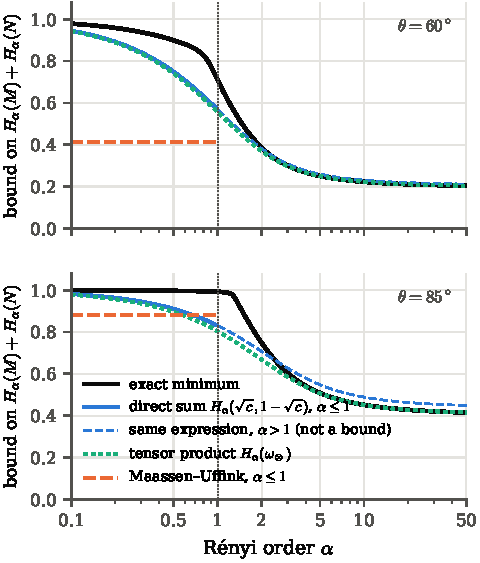
\includegraphics[width=\columnwidth]{renyi_family.pdf}
  \caption{Bounds on $H_\alpha(M)+H_\alpha(N)$ across the R\'enyi family for
  $\theta=60^\circ$ (top) and $\theta=85^\circ$ (bottom). Black: exact minimum.
  Blue: direct-sum bound $H_\alpha(\sqc,1-\sqc)$ of Corollary~\ref{cor:direct},
  valid for $\alpha\le1$; its thin dashed continuation for $\alpha>1$ is not a
  bound and eventually exceeds the exact minimum. Green (dotted):
  tensor-product bound $H_\alpha(\omtimes)$ of Corollary~\ref{cor:tensor}.
  Orange (dashed): MU, valid for $\alpha\le1$. The dotted vertical line marks
  the Shannon case $\alpha=1$.}
  \label{fig:renyi}
\end{figure}

Finally, MU is one member of a family $H_\alpha(p)+H_\beta(q)\ge-\log_2c$ with
$1/\alpha+1/\beta=2$~\cite{MaassenUffink1988}, which includes the pair
$H_\infty(p)+H_{1/2}(q)\ge-\log_2c$ of min- and max-entropy. Majorization
relations of the form~\eqref{eq:maj-UR} are symmetric under the exchange of $p$
and $q$ and therefore yield such mixed-order relations only indirectly, through
the monotonicity of $H_\alpha$ in $\alpha$.

% ===========================================================================
\section{General two-outcome qubit POVMs}
\label{sec:povm}
% ===========================================================================

For POVMs, the partial sums of the direct-sum relation are largest eigenvalues
of sums of effects, $S_k=\max_{|J|=k}\lambda_{\max}\bigl(\sum_{j\in J}F_j\bigr)$,
where the $F_j$ run over the effects of both
measurements~\cite{Baek2019} (see also
Refs.~\cite{RPZ2014,RasteginZyczkowski2016,Bosyk2014}); Baek \emph{et al.}
evaluated them for unbiased unsharp qubit observables~\cite{Baek2019}. For
two-outcome qubit POVMs the maximization can be carried out in closed form for
arbitrary bias, and the resulting vector turns out to be ordered, hence optimal.

Let $M=\{E_0,E_1\}$ with parameters $(\mu,\eta,\hat a)$ and $N=\{F_0,F_1\}$ with
$(\nu,\zeta,\hat b)$, as in Eq.~\eqref{eq:povm}. Then
$p=\frac12\bigl(1+\mu+\eta\,\hat a\cdot\vecr,\;1-\mu-\eta\,\hat a\cdot\vecr\bigr)$, and
similarly for $q$.

\begin{theorem}
\label{thm:povm}
Define
\begin{align}
  \kappa&=\max\{|\mu|+\eta,\;|\nu|+\zeta\},\\
  \Lambda&=\max_{s,t=\pm1}\bigl[s\mu+t\nu+|s\eta\,\hat a+t\zeta\,\hat b|\bigr].
\end{align}
Then $p(\rho)\oplus q(\rho)\maj\omplus$ for all $\rho$, where
\begin{equation}
  \omplus=\tfrac12\bigl(1+\kappa,\;1+\Lambda-\kappa,\;1+\kappa-\Lambda,\;1-\kappa\bigr)
  \label{eq:om-povm}
\end{equation}
is the optimal majorization bound.
\end{theorem}

\begin{proof}
The largest single outcome probability is
$\max_\rho\frac12\bigl(1+|\mu+\eta\,\hat a\cdot\vecr|\bigr)=\frac12(1+|\mu|+\eta)$ for $M$,
so $S_1=\frac12(1+\kappa)$; likewise the smallest is $\frac12(1-\kappa)$, so
$S_3=2-\frac12(1-\kappa)$. For $S_2$, a pair within one distribution sums to $1$,
while a cross pair gives, by Eq.~\eqref{eq:support},
\begin{multline}
  \max_\rho\bigl[1+\tfrac12\bigl(s(\mu+\eta\,\hat a\cdot\vecr)+t(\nu+\zeta\,\hat b\cdot\vecr)\bigr)\bigr]\\
  =1+\tfrac12\bigl[s\mu+t\nu+|s\eta\hat a+t\zeta\hat b|\bigr].
\end{multline}
Choosing $s=\operatorname{sgn}\mu$, $t=\operatorname{sgn}\nu$ shows $\Lambda\ge0$,
so $S_2=1+\frac12\Lambda$. The increments of $(S_k)$ are the entries of
Eq.~\eqref{eq:om-povm}. They are non-increasing iff $\kappa\le\Lambda\le2\kappa$.
The upper inequality follows from the triangle inequality,
$\Lambda\le|\mu|+|\nu|+\eta+\zeta\le2\kappa$. For the lower one, let $\rho^\ast$
attain $S_1$ via an outcome of, say, $M$; then
$S_2\ge S_1+\max_jq_j(\rho^\ast)\ge S_1+\frac12$, i.e., $\Lambda\ge\kappa$.
Lemma~\ref{lem:sup} completes the proof.
\end{proof}

For projective measurements $\kappa=1$, $\Lambda=2\sqc$ and
Eq.~\eqref{eq:om-povm} reduces to Eq.~\eqref{eq:omplus}. For unbiased
measurements ($\mu=\nu=0$),
$\Lambda=(\eta^2+\zeta^2+2\eta\zeta|\hat a\cdot\hat b|)^{1/2}$, in agreement with
Ref.~\cite{Baek2019}. If moreover $\eta=\zeta$, then
$\omplus=\eta\,(1,\sqc,1-\sqc,0)+\frac{1-\eta}{2}(1,1,1,1)$: such measurements
are noisy versions of sharp ones~\cite{Busch1986,Baek2019}, and the achievable
statistics, their supremum and the saturating states are those of the sharp case
mixed with the uniform vector. For unequal sharpness or nonzero bias, $\omplus$
is not of this form, and the relevant geometric quantities are the lengths
$|\eta\hat a\pm\zeta\hat b|$ rather than the overlap $c$.

\emph{Uncertainty versus incompatibility.}---For unbiased POVMs the vectors
$\eta\hat a\pm\zeta\hat b$ that determine $\Lambda$ also decide joint
measurability: the pair is jointly measurable if and only if
$|\eta\hat a+\zeta\hat b|+|\eta\hat a-\zeta\hat b|\le2$~\cite{Busch1986,HMZ2016}.
The two notions are nevertheless distinct. For orthogonal axes and
$\eta=\zeta\le1/\sqrt2$ the measurements are jointly measurable, yet
$S_2=1+\eta/\sqrt2$ stays below the value $1+\eta$ that would be reached if both
outcome distributions could be sharpened at once, and $\omplus$ is not attained,
being a noisy version of the sharp bound (Proposition~\ref{prop:attain}).
Majorization uncertainty relations therefore quantify preparation uncertainty,
which persists in the absence of measurement incompatibility.

As a corollary, $H(p)+H(q)\ge-\sum_k\omega_k\log_2\omega_k$ for all
two-outcome qubit POVMs. Figure~\ref{fig:povm} shows that this bound tracks
the exact minimum over the whole range of sharpness, becoming exact in the
trivial limit $\eta\to0$.

\begin{figure}[t]
  \centering
  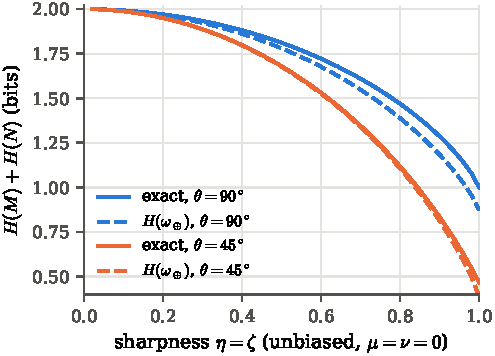
\includegraphics[width=\columnwidth]{povm.pdf}
  \caption{Unsharp measurements ($\mu=\nu=0$, $\eta=\zeta$): exact minimum of
  $H(M)+H(N)$ (solid) and the bound from Theorem~\ref{thm:povm} (dashed) for
  Bloch angles $90^\circ$ and $45^\circ$.}
  \label{fig:povm}
\end{figure}

% ===========================================================================
\section{Binary projective measurements in dimension \texorpdfstring{$d$}{d}}
\label{sec:dimd}
% ===========================================================================

The qubit analysis already contains the general binary projective case.

\begin{theorem}
\label{thm:dimd}
Let $M=\{P,\mathbb{1}-P\}$ and $N=\{Q,\mathbb{1}-Q\}$ be projective measurements on
$\mathbb{C}^d$ and $c=\max_{i,j}\|P_iQ_j\|_\infty^2$. Then
Theorems~\ref{thm:direct} and~\ref{thm:tensor} hold verbatim, and $\omplus$ is
attained if and only if $c=1$.
\end{theorem}

\begin{proof}
By Jordan's lemma~\cite{Halmos1969}, which is also the standard tool for
entropic uncertainty relations of binary measurements~\cite{KTW2014},
$\mathbb{C}^d$ decomposes into mutually orthogonal subspaces $\mathcal{H}_b$ of
dimension one or two, each invariant under $P$ and $Q$. On a two-dimensional
block, $P$ and $Q$ act as rank-one projectors, i.e., as a pair of qubit
measurements with overlap $c_b$; on a one-dimensional block they have a common
eigenvector, and we set $c_b=1$. Since $P$ and $Q$ are block diagonal,
$p(\rho)\oplus q(\rho)=\sum_b\lambda_b\,p_b\oplus q_b$ with
$\lambda_b=\tr(\rho\Pi_b)$ and $p_b,q_b$ the statistics of the normalized block
state $\Pi_b\rho\Pi_b/\lambda_b$. Each $p_b\oplus q_b\maj\omplus(c_b)\maj\omplus(c)$,
because $\omplus$ increases in the majorization order with $c$ and
$c=\max_bc_b$. Since $\{v:v\maj\omega\}$ is convex, $p\oplus q\maj\omplus(c)$;
optimality follows by embedding the maximizing qubit states of a block with
$c_b=c$. For the tensor product, $p_iq_j\le(\frac{p_i+q_j}{2})^2$ with
$p_i+q_j\le\lambda_{\max}(P_i+Q_j)=1+\|P_iQ_j\|\le1+\sqc$; $S_1=w$ is attained in
a block with $c_b=c$, and $S_2=1$ by any state in the range of $P$. Finally, if
$c<1$, a state with $L_1(p\oplus q)=1$ lies in the range of some $P_i$ (or
$Q_j$); then $q_j=\tr(\rho P_iQ_jP_i)\le\|P_iQ_j\|^2\le c$ for all $j$, so
$L_2(p\oplus q)\le1+c<1+\sqc$ and $\omplus$ is not attained. If $c=1$, the
ranges of some $P_i$ and $Q_j$ intersect and a common eigenvector attains
$\omplus=(1,1,0,0)$.
\end{proof}

In particular, all bounds of Sec.~\ref{sec:entropic} hold for binary projective
measurements in any dimension with $c=\max_{i,j}\|P_iQ_j\|^2$, and the
min-entropy bound remains tight.
For arbitrary POVMs in any dimension, the eigenvalue formula for $S_k$ quoted in
Sec.~\ref{sec:povm}, together with Lemma~\ref{lem:sup}, gives an exact
numerical procedure, which we use to verify Theorems~\ref{thm:povm}
and~\ref{thm:dimd} independently (Appendix~\ref{app:numerics}).

% ===========================================================================
\section{Discussion}
\label{sec:discussion}
% ===========================================================================

For binary measurements the majorization approach to uncertainty can be
carried out completely. The achievable statistics form an affine image of an
ellipse, and a single four-component vector, determined by the overlap $c$ (or,
for POVMs, by $\kappa$ and $\Lambda$), is their least upper bound in the
majorization lattice, for the direct sum as well as for the tensor product.
This is the unified perspective that majorization offers: one vector controls
every Schur-concave uncertainty measure at once.

The comparison with entropy-specific relations shows what this unification
costs. Because the supremum is not the statistics of any state when the
measurements do not commute, the induced bound is strict for every strictly
Schur-concave measure, and it becomes exact only at the extreme orders
$\alpha=0$ and $\alpha=\infty$. Against a generic scalar relation such as MU,
on the other hand, the majorization bounds are strong: the direct-sum Shannon
bound beats MU for Bloch angles below $81.3^\circ$ and is asymptotically tight
in ratio as the measurements approach compatibility, precisely where MU is
weakest. Among the two forms, the direct sum is preferable for $\alpha\le1$,
while only the tensor product survives for large $\alpha$.

Several questions remain open.
(i) \emph{Tensor bounds for POVMs.} The AM--GM step of Theorem~\ref{thm:tensor}
is no longer tight for biased or unequally sharp measurements; the optimal
$\omtimes$ then requires maximizing products of affine functions over
$\mathcal{E}_\theta$, and the least concave majorant in Lemma~\ref{lem:sup} may
become non-trivial.
(ii) \emph{Binary POVMs in dimension $d$.} Jordan's lemma does not apply to
pairs of effects directly. A Naimark dilation~\cite{Peres1993} turns them into
projectors, but only product inputs are allowed, so Theorem~\ref{thm:dimd} does
not apply as it stands.
(iii) \emph{More measurements.} For three or more binary measurements the
partial sums involve signed sums of several Bloch vectors, and the lattice
structure of the bound becomes genuinely relevant.
(iv) \emph{Mixed orders.} It remains open whether majorization can be adapted
to yield relations such as $H_\infty(p)+H_{1/2}(q)\ge-\log_2c$.

\begin{acknowledgments}
The author thanks Marcelo Ciappina and Gilad Gour for guidance and discussions.
% \todo{funding information}
\end{acknowledgments}

\appendix

% ===========================================================================
\section{Numerical methods and code}
\label{app:numerics}
% ===========================================================================

All results were checked with the accompanying Python code (\texttt{code/}):
\begin{itemize}
  \item \texttt{majorization.py}: POVM parametrization, Lorenz curves, the lattice
    supremum via least concave majorants~\cite{CicaleseVaccaro2002}, the
    analytic bounds of Theorems~\ref{thm:direct}, \ref{thm:tensor}
    and~\ref{thm:povm} and Corollaries~\ref{cor:direct}--\ref{cor:tensor}, the
    eigenvalue characterization $S_k=\max_{|J|=k}\lambda_{\max}(\sum_{j\in J}F_j)$,
    and exact minima of R\'enyi and Tsallis entropy sums.
  \item \texttt{verify\_bounds.py}: compares the closed forms with (a) lattice
    suprema over $1.8\times10^5$ grid states (maximal deviation $<10^{-4}$), and
    (b) the eigenvalue characterization for 200 random qubit POVM pairs and for
    150 random pairs of projectors of rank $d/2$ in dimensions $d=2,4,6$, all
    with $c<1$ (deviation $<10^{-14}$). Pairs with a common eigenvector, which
    always occur for odd $d$ or unequal ranks, have $c=1$ and are checked
    separately. The script also checks Propositions~\ref{prop:attain}
    and~\ref{prop:compare}, Corollaries~\ref{cor:direct}--\ref{cor:tensor},
    Theorem~\ref{thm:tight}, the critical angle $\bar\theta$, and the jointly
    measurable example of Sec.~\ref{sec:povm}.
  \item \texttt{make\_figures.py}: generates Figs.~\ref{fig:ellipse}--\ref{fig:povm}.
\end{itemize}
The exact entropy minima are obtained by a dense grid over the great circle in
$\mathrm{span}\{\mhat,\nhat\}$ refined by Nelder--Mead. This reduction is justified
by Lemma~\ref{lem:ellipse}: the Shannon entropy is concave in $(x,y)$ and is
therefore minimized on the boundary of $\mathcal{E}_\theta$. For unbiased
measurements, moving $\vecr$ outwards makes both $p$ and $q$ more ordered, so the
same holds for every R\'enyi and Tsallis entropy.

\bibliography{references}

\end{document}
